\subsection{Mašīnmācīšanās modelis}

    Mašīnmācīšanās modeļa izstrādi ir iespējams sadalīt vēl divās daļās: modeļa trennēšana un modeļa
    implementācija tīmekļa aplikācijā.

    Sākotnēji tika veikta modeļa trennēšana, bet vēl pirms tā tika veikta izpēte par to kādi gatavi
    ietvari jau eksistē \texttt{C\#} ekosistēmā. Pēc vairāku ietvaru izpētes kā \texttt{PyTorch.NET},
    \texttt{Keras.NET}, \texttt{ML.NET} un \texttt{CNTK}. Sākumā bija plānots izmantot \texttt{CNTK},
    bet izpētes processā tika secināts, ka Microsoft ir pārtraukuši atbalstu \texttt{CNTK} un vairs
    to neuzlabos un neatjaunos, tapēc beigas tika izvēlēts \texttt{ML.NET}.

    Attiecīgi tika izveidota programma, kas apmāca modeli izmantojot \texttt{MNIST} datu kopu un
    šīs programmas darbība ir aprakstīta \ref{ml:train}~attēlā.

    \begin{figure}[H]
        \centering
        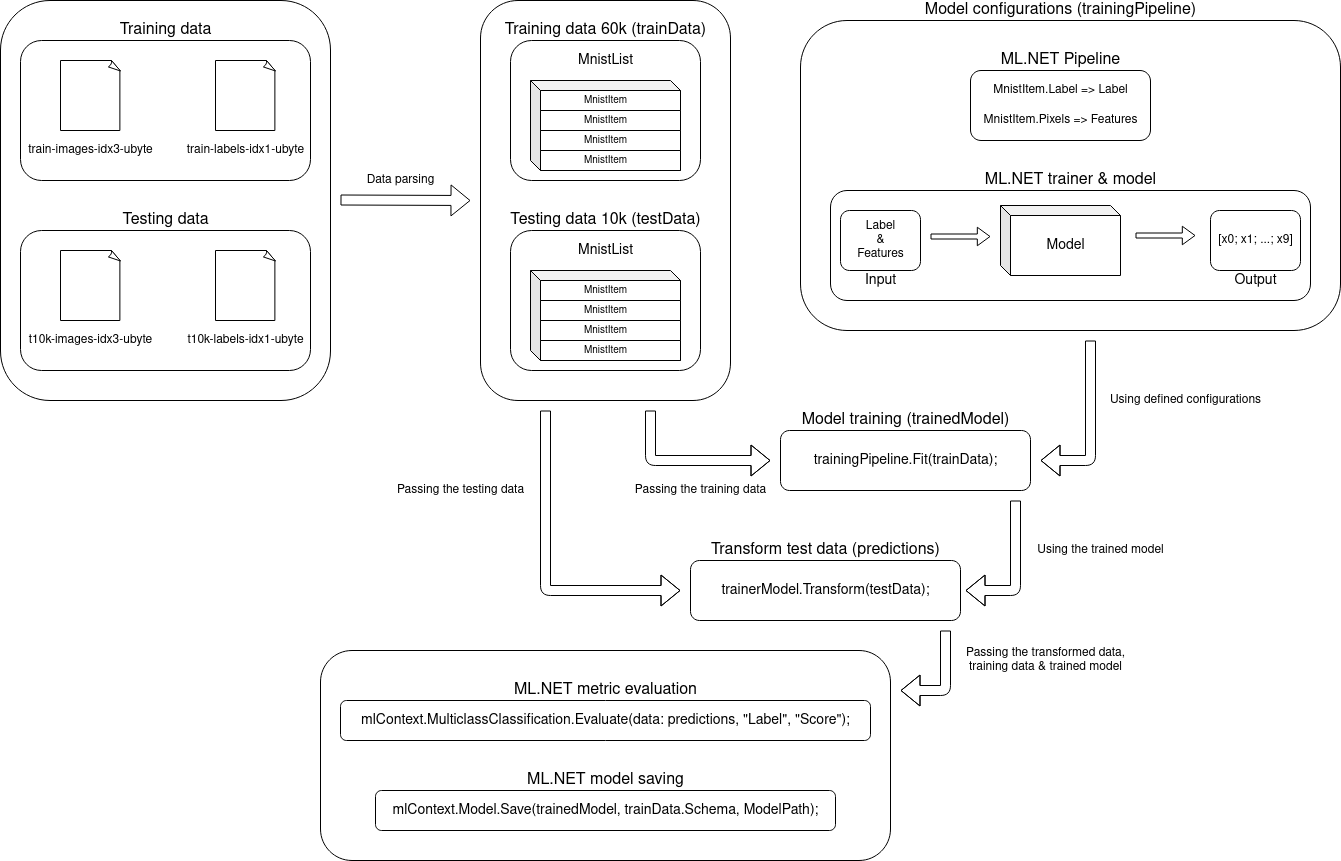
\includegraphics[width=15cm]{VPL-ML.png}
        \caption{ML modeļa trennēšanas diagramma}
        \label{ml:train}
    \end{figure}

    Sākumā tika iegūti \texttt{MNIST} dati no "THE MNIST DATABASE" [insert reference]. Tie ir 4 bināri
    faili un tos diagrammā var redzēt "Training data" un "Testing data" kvadrātos. Pēc datu iegūšanas
    tika izveidots datu parser funkcija, kas ielasa visus datus atmiņā un sadala to pa klasēm un šīs
    klases ir "MnistList" un "MnistItem". Izmantojot \texttt{ML.NET} tiek nodefinēta konfigurācija
    prieks \texttt{ML.NET} "pipeline". Konfigurācijā ietilpst mainīgo sasaistīšana un modeļa veida
    definēšana. Pēc konfigurācijas nodefinēšanas un datu ielasīšanas tiek trennēts modelis izmantojot
    \mintinline{csharp}{.Fit()} metodi. Pēc modeļa trennēšanas ir nepieciešams pārbaudīt cik labi šis
    modelis ir uztrennēts, tapēc tiek veiktas transformācijas uz datiem, kuri tika izmantoti modeļa
    trennēšanā, izmantojot \mintinline{csharp}{.Transform()} metodi, un izmanotjot šos datus tiek
    veikta modeļa izvērtēšana izmantojot \mintinline{csharp}{.Evaluate()} metodi. Pēdejais solis ir
    to saglabāt. Tas tiek izdarīts izmantojot \mintinline{csharp}{.Save()} metodi.

    Rezultātā tika iegūts modelis, kuru metriku rezultāti ir redzami \ref{ml:metrics}~attēlā.

    \begin{figure}[H]
        \centering
        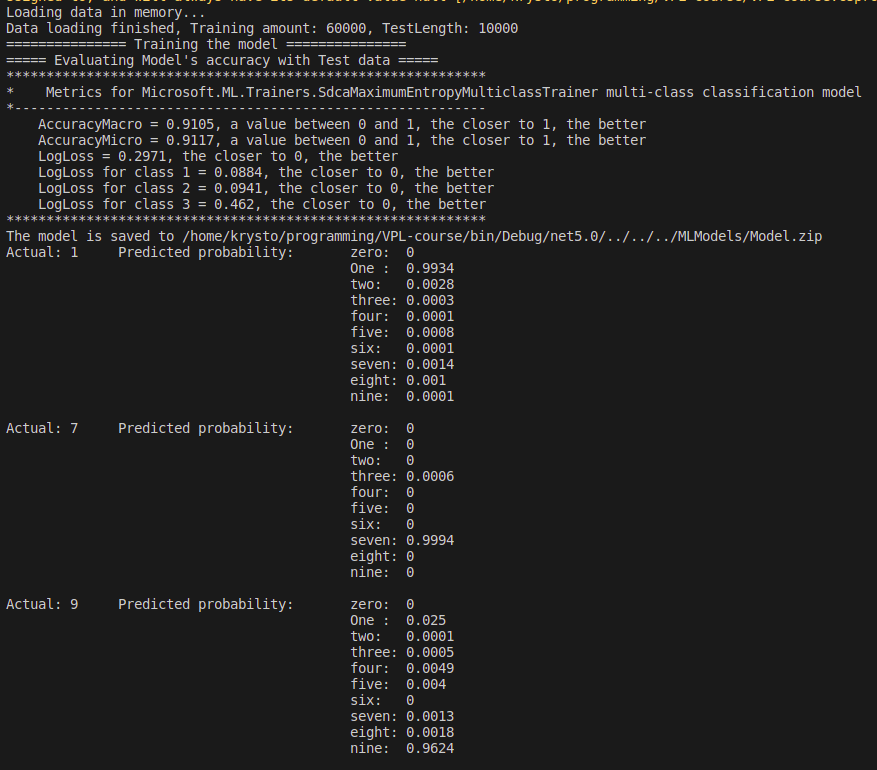
\includegraphics[width=13cm]{training-sc-v2.png}
        \caption{ML modeļa metriku rezultāti}
        \label{ml:metrics}
    \end{figure}

    Kad modelis bija izveidots, tad to bija nepieciešams implementēt tīmekļa aplikācijā. Tika izveidota
    \mintinline{csharp}{MnistClassificator} klase, kurā tika izveidota metode
    \mintinline{csharp}{public float[] Analyze(byte[] image)}, kurai ir iespējams padot bināru virkni,
    kas attiecīgi tiek padota izveidotam modelim, kas atgriež virkni ar float vērtībām. Šīs vērtības
    reprezentē procentuālās vērtības ciparu klasēm.
